
\section{Introduction}

\subsection{Objectives}

\begin{itemize}
\item Learn the difference between compiled and interpreted programming languages.
\item Learn basic facts about Python and its powerful accompanying libraries.
\item Understand how Python programming works in the web browser.
\item Write and run your first Python program.
\end{itemize}

\subsection{Compiled and interpreted programming languages}

Let us explain the main difference between {\em compiled} and {\em interpreted} programming languages. 
{\em Compilation} is a process where human-readable {\em source code (text)} is translated by
means of a {\em compiler} and a {\em linker}
into a {\em binary (executable) file} which then can be run on the concrete computer. The same 
source code, compiled on different hardware architectures, yields different binaries. 

{\em Interpreted (scripting)} programming languages are more recent than the compiled ones. 
A program that is written using an interpreted language is "read" (parsed) at runtime -- it is 
not compiled and there are no binaries. Programs 
written in compiled languages are usually more efficient than programs written in the interpreted 
ones because the former take better advantage of the underlying hardware. On the other hand,
interpreted languages are usually more universal and easier to use. Compiled 
programming languages include Pascal, C, C++, Fortran, and many others. Few examples of interpreted 
languages are Python, Lua, Perl and Ruby. 

\subsection{Basic facts about Python}

Python is a powerful modern programming language that is used in many areas of 
engineering and science. Its interpreted character along with a very intuitive syntax make Python an 
ideal language for beginners. 

Python was conceived in the late 1980s and its implementation was started in December 1989
by Guido van Rossum at CWI in the Netherlands. Rossum also gave it a name originated
in his favorite television series {\em Monty Python's Flying Circus}.
Python 2.0 was released in October 2000 and Python 3.0 in December 2008. Python was
awarded the TIOBE {\em Programming Language of the Year} award twice (2007, 2010), which is 
given to the language with the greatest growth in popularity over the course of a year.

Python is a multi-paradigm programming language. Rather than forcing programmers to 
adopt a particular style of programming, it permits several styles: {\em structured (procedural) 
programming} and {\em object-oriented programming} are fully supported, and there are a number 
of language features which support {\em functional programming}. 

In this short course you will 
learn the most important aspects of the language and be able to 
write a wide range of programs by yourself. Depending on your objectives, this course 
might be all you will ever need. We hope that you will like Python and want
to learn more -- and there is much more to learn out there. References to materials
covering more advanced topics and object-oriented programming are given in Section \ref{sec:adv}.

\subsection{Libraries - the strong companion of Python}

Python comes with a powerful {\em standard library} that contains plentiful functionality
to ease work with constants, types, functions, exceptions, strings, data, 
mathematics, cryptography, parallel processing and other things. 
Python also has a number of scientific libraries. Most important of them are Scipy, 
Numpy, Pylab, Matplotlib, and Sympy. Exploring Python libraries will be a significant 
part of this course. 

\subsection{How does Python programming in work in the web browser?}

In the browser, Python code is typed into one or more input cells in the {\em Python worksheet}. 
The code is sent (as a text string) to a remote server where it is interpreted, and the 
results are sent back to your computer / laptop / tablet, and displayed in your web 
browser.  Let's try this!

\subsection{Launching a Python project}

There are multiple ways to launch a Python project. First, it is 
possible to clone and experiment with many existing displayed Python 
projects via File Manager $\rightarrow$ 
Project $\rightarrow$ Clone. New (empty) Python project can be launched via 
the {\em Programming} menu or via File Manager $\rightarrow$ 
Project $\rightarrow$ New $\rightarrow$ Python. An empty Python worksheet
is shown in Fig. \ref{fig:python}.

\newpage
\begin{figure}[!ht]
\begin{center}
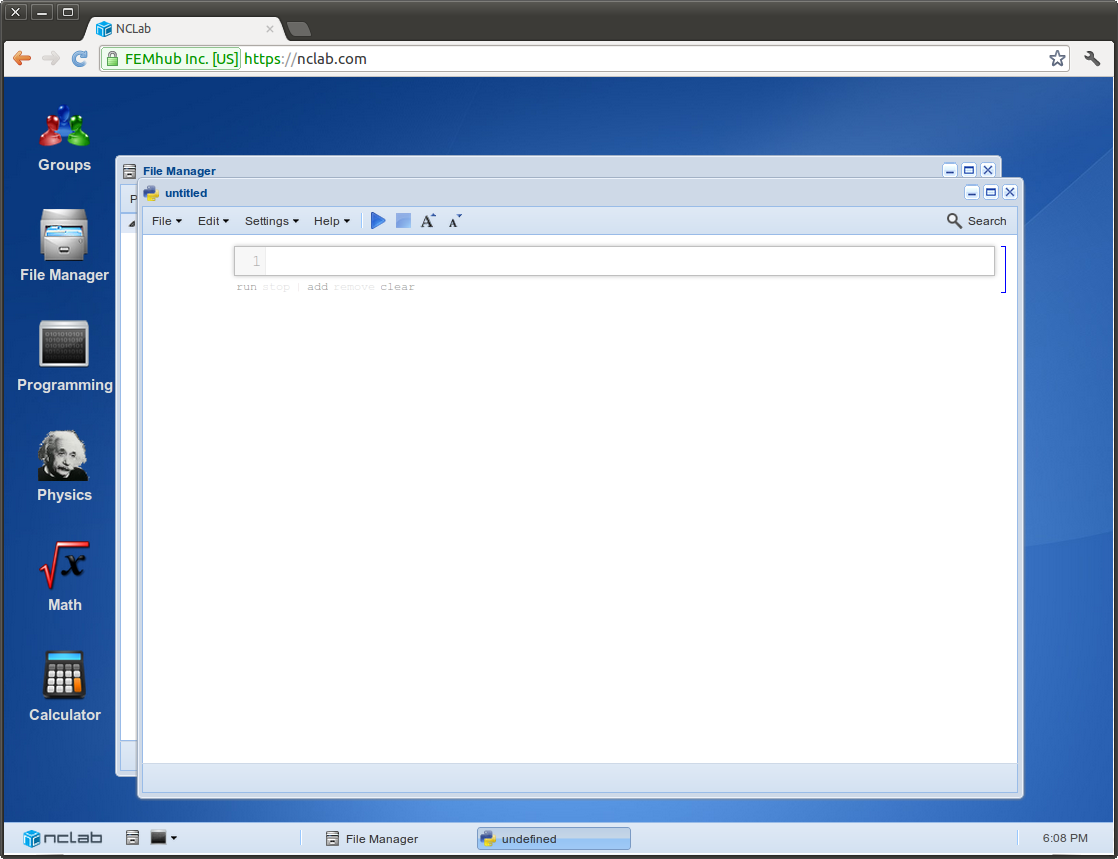
\includegraphics[width=0.9\textwidth]{imgp/python.png}
\end{center}
\vspace{-2mm}
\caption{Launching a new Python project.}
\label{fig:python}
\end{figure}


\subsection{Hello, World!}

Click into the input cell and type {\tt print "Hello, World!"}.
Then click on {\tt run} link under the input cell, and the text 
"Hello, World!" will be displayed 
in a new yellow {\em output cell} as shown in Fig. \ref{fig:python-2}.

\newpage

\begin{figure}[!ht]
\begin{center}
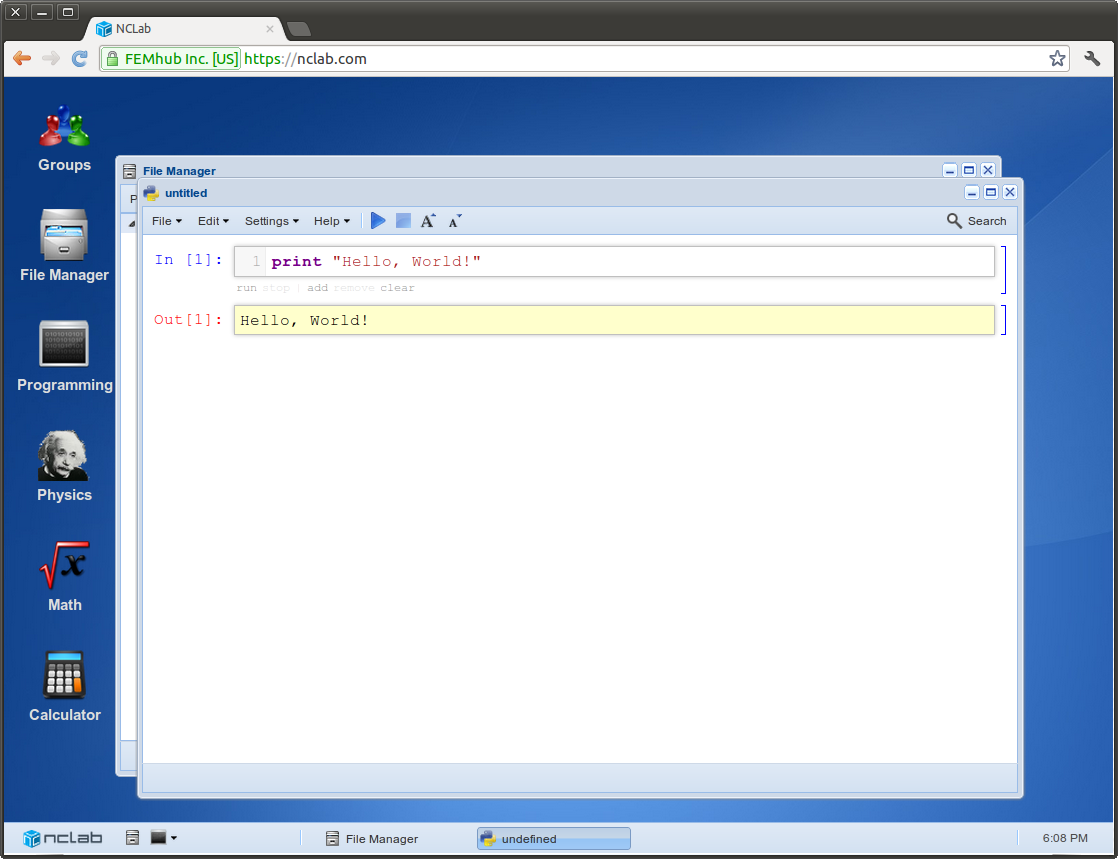
\includegraphics[width=0.9\textwidth]{imgp/python-2.png}
\end{center}
\vspace{-2mm}
\caption{Response received from the cloud is shown in a yellow output cell.}
\label{fig:python-2}
\end{figure}

\subsection{Input, output and text cells}

The Python worksheet contains three types of cells - input cells, output cells, 
and descriptive text cells. Input cells as well as text cells can be added via 
the {\em Edit} menu. New input cells can be also added easily by clicking on {\tt add} under
an existing input cell. Input cells and text cells can be removed by clicking on 
{\tt remove} under them. The easiest way to remove a selected output cell is to 
click on it with the mouse and press DELETE on the keyboard. 
All output cells can be removed at once via {\em Remove all output} in the {\em Edit} menu. 

\subsection{Various ways to run programs}

Pressing the blue arrow button will run all input cells in the project. Clicking 
on {\tt run} under an input cell will run only the contents of that input cell. 
Same effect can be achieved by holding CTRL and pressing ENTER. Holding SHIFT
and pressing ENTER will evaluate the current input cell and create an additional one
under it.

\subsection{\ \ Review questions}

In all multiple-choice questions in this textbook, one or more answers can be correct. 
\begin{enumerate}
\item What is the difference between a compiled and a scripting programming language?
\begin{enumerate}
\item[A1] Programs written in compiled languages are binary files. 
\item[A2] Compiled languages are easier to use than the scripting ones.
\item[A3] Programs written in scripting languages are usually more efficient than programs 
          written in the compiled ones.
\item[A4] Scripting languages do not require a compiler.
\end{enumerate}
\item What languages take better advantage of the underlying hardware architecture
      and why?
\begin{enumerate}
\item[A1] Scripting languages because they are less hardware-dependent.
\item[A2] Compiled languages because the executable files are tailored 
          to the concrete hardware.
\item[A3] Compiled languages because  they do not require a linker.
\item[A4] Scripting languages because they do not require a compiler.
\end{enumerate}
\item Give three examples of compiled programming languages.
\begin{enumerate}
\item[A1] Fortran, C++ and Lua.
\item[A2] Python, Ruby and C.
\item[A3] C, C++ and Fortran.
\item[A4] Python, Lua and Perl.
\end{enumerate}
\item Give three examples of interpreted programming languages.
\begin{enumerate}
\item[A1] Pascal, Perl and Python.
\item[A2] Lua, C and C++.
\item[A3] Perl, Python and Ruby. 
\item[A4] C, C++ and Fortran.
\end{enumerate}
\item Where does the name "Python" of the programming language come from?
\begin{enumerate}
\item[A1] The snake, {\em Python regius}.
\item[A2] TV show in Great Britain.
\item[A3] Recognized brand name of remote start systems.
\item[A4] Recognized brand name of aquarium products.
\end{enumerate}
\item When was the implementation of Python started?
\begin{enumerate}
\item[A1] 1989
\item[A2] 1995
\item[A3] 2000
\item[A4] 2005
\end{enumerate}
\item Name three programming styles that Python permits.
\begin{enumerate}
\item[A1] Compiled, interpreted, scripting.
\item[A2] Structured, object-oriented, functional.
\item[A3] Procedural, object-oriented, binary.
\item[A4] Good, bad, ugly.
\end{enumerate}
\item How can displayed Python projects be cloned?
\begin{enumerate}
\item[A1] In Python worksheet through the {\em File} menu.
\item[A2] Through File Manager's {\em Project} menu.
\item[A3] Using the icon {\em Displayed projects} on Desktop.
\item[A4] Python projects cannot be cloned.
\end{enumerate}
\item How can new Python project be launched?
\begin{enumerate}
\item[A1] Through the {\em Programming} menu.
\item[A2] Through File Manager's {\em Settings} menu.
\item[A3] Through File Manager's {\em Project} menu.
\item[A4] Through the Math module.
\end{enumerate}
\item How are Python programs processed?
\begin{enumerate}
\item[A1] They are translated into Javascript and run as a standard web browser application.
\item[A2] They are interpreted on a remote server.
\item[A3] They are interpreted on your PC computer / laptop / tablet.
\item[A4] They are translated into Flash.
\end{enumerate}
\item What are the types of cells that a Python worksheet can contain?
\begin{enumerate}
\item[A1] Error message cells.
\item[A2] Output cells.
\item[A3] Input cells.
\item[A4] Descriptive text cells.
\end{enumerate}
\item How can all input cells in a Python worksheet be evaluated at once?
\begin{enumerate}
\item[A1] By typing Evaluate in the last input cell and hitting ENTER.
\item[A2] By clicking on {\tt run} under the last input cell.
\item[A3] By clicking on {\em Evaluate all} in the {\em File} menu. 
\item[A4] By clicking on the blue arrow button in the menu.
\end{enumerate}
\item How can a single input cell be evaluated?
\begin{enumerate}
\item[A1] By clicking on {\tt save} under the input cell.
\item[A2] By clicking on the blue arrow button in the menu.
\item[A3] By clicking on {\tt run} under the input cell.
\item[A4] By clicking on the blue square button in the menu.
\end{enumerate}
\item What is the way to add a new input cell?
\begin{enumerate}
\item[A1] Click on {\tt add} under an input cell. 
\item[A2] Click on {\em New} in the {\em File} menu.
\item[A3] Click on the larger "A" icon in the menu.
\item[A4] Click on {\em New input cell} in {\em Edit} menu.
\end{enumerate}
\item How can a new text cell be added?
\begin{enumerate}
\item[A1] Click on {\tt add} under an input cell. 
\item[A2] Click on {\em New text cell} in the {\em Edit} menu.
\item[A3] Click on {\em New} in the {\em File} menu.
\item[A4] Click on the smaller "A" icon in the menu.
\end{enumerate}
\item What is the way to remove an input cell or a text cell?
\begin{enumerate}
\item[A1] Click on {\tt remove} under the cell. 
\item[A2] Click on {\tt clear} under the cell. 
\item[A3] Click on {\em Clear active cell} in the {\em Edit} menu.
\item[A4] Click on {\em Close} in the {\em File} menu.
\end{enumerate}
\item How can an input cell be evaluated without using the mouse?
\begin{enumerate}
\item[A1] Hold CTRL and press ENTER.
\item[A2] Hold SHIFT and press ENTER.
\item[A3] Press ENTER twice.
\item[A4] Press CTRL + ALT + SHIFT.
\end{enumerate}
\item Which of the following are scientific libraries for Python?
\begin{enumerate}
\item[A1] GNU Scientific Library.
\item[A2] Numpy.
\item[A3] Scipy.
\item[A4] Sympy.
\end{enumerate}
\end{enumerate}

\subsection{\ \ Exercises}

\begin{enumerate}
\item Write a Python program that prints your name. Run it by clicking on the blue arrow button.
\item Write a Python program that prints the name of your favorite animal. 
      Run it by clicking on {\tt run} under the input cell.
\item Write a Python program that prints the name of your favorite singer 
      or music band. Run it without using the mouse.
\end{enumerate}

\section{Using Python as a calculator}

\subsection{Objectives}

\begin{itemize}
\item Learn how to do both simple and advanced math operations in the Python worksheet.
\end{itemize}
As you certainly noticed, there is a small pocket calculator for quick anytime 
calculations. In this section we will see that also the Python worksheet can be 
used as a calculator, which is backed up by hundreds of processors and much more powerful indeed.

\subsection{Addition, subtraction}

Launch a new Python project and in the input cell type:

\begin{verbatim}
3 + 6
\end{verbatim}
Then click on the {\tt run} link under the input cell. The output should be displayed quickly:

\begin{verbatim}
9
\end{verbatim}
You can add real numbers too,
\begin{verbatim}
3.2 + 6.31
\end{verbatim}
Output:

\begin{verbatim}
9.51
\end{verbatim}
Two numbers can be subtracted as follows,

\begin{verbatim}
7.5 - 2.1
\end{verbatim}
Output:

\begin{verbatim}
5.4
\end{verbatim}
\subsection{Multiplication}
Multiplication is done using the '{\tt *}' symbol as in

\begin{verbatim}
3 * 12
\end{verbatim}
Output:

\begin{verbatim}
36
\end{verbatim}
Of course, real numbers can be multiplied as well:

\begin{verbatim}
3.7 * 12.17
\end{verbatim}
Output:

\begin{verbatim}
45.029
\end{verbatim}
\subsection{Division}
With division, we need to be a bit careful. Look at this:

\begin{verbatim}
30 / 5
\end{verbatim}
Output:

\begin{verbatim}
6
\end{verbatim}
And then look at this:

\begin{verbatim}
33 / 5
\end{verbatim}
Output:

\begin{verbatim}
6
\end{verbatim}
In all major computer languages including C, C++, Fortran, Python and 
others:\\

\begin{center}
\framebox{\color{red}\bf The result of division of two integers is an integer!}
\end{center}

\vspace{4mm}
\noindent
So, when dividing two integers, everything behind the decimal point is lost.
In order to stay on the safe side, 
before you perform division of two numbers, always convert at least one of them
to a real number. This is simple: While {\tt 5} is an integer, {\tt 5.}
and {\tt 5.0} are reals. It is also possible to 
say {\tt float(5)}. In fact this is the best way since it also works for 
variables. Such as, when we are dividing {\tt a / b}, to make sure that 
the result will be correct also for integers, we type {\tt float(a) / b}. 
When at least one number is a real, then the result of the division is a real.   
Variables will be discussed shortly.

\subsection{Powers}
Sometimes we need to use exponents, such as in $2^4$. Python has a double-star
symbol {\tt **} for this:

\begin{verbatim}
2**4
\end{verbatim}
Output:

\begin{verbatim}
16
\end{verbatim}
\subsection{Modulo}
The last of the common arithmetic operations is {\em modulo}. Recall that this is the remainder 
after integer division. In Python modulo is done using the per cent symbol:

\begin{verbatim}
6 % 4
\end{verbatim}
Output:

\begin{verbatim}
2
\end{verbatim}
Of course, one can use brackets:

\begin{verbatim}
5 * (7 - 3)
\end{verbatim}
Output:

\begin{verbatim}
20
\end{verbatim}
\subsection{Order of operations}
Python respects the standard order of operations:

\begin{itemize} 
\item Round brackets have the highest priority,
\item then exponentiation, 
\item then multiplication and division (same priority),
\item the lowest priority have addition and subtraction.
\end{itemize}
Note that no other brackets such as {\tt \{ \}} and {\tt [ ]} are 
admissible in mathematical expressions since they have a different 
function in the programming language.

To illustrate the priority of operations, we can try the following:

\begin{verbatim}
3**4 / 27 * 5 + 3 * 5
\end{verbatim}
Output:

\begin{verbatim}
30
\end{verbatim}
\subsection{Using empty characters makes you code better readable}
Your code will be much better readable when you use empty
characters on either side of arithmetic symbols, as well as 
after commas. Hence, you should never write things like {\tt 3**4/27*5+3*5}.

\subsection{Using mathematical functions}

In order to calculate square roots, exponentials, sins, cosins, tangents, and all other 
simple functions, the best way is to import Numpy. Numpy is a standard Python library 
for numerical computations. To import it, just include the following 
line in your code:

\begin{verbatim}
from numpy import *
\end{verbatim}
Here the symbol {\tt *} stands for "everything". If you wanted to import just one or two 
functions, you could do that as well by just giving their names, separated by commas. 

After Numpy is imported, we can calculate for example $e^2$:

\begin{verbatim}
exp(2)
\end{verbatim}
Output:
\begin{verbatim}
7.3890560989306504
\end{verbatim}
Elementary functions (and constants) that one can import from Numpy are listed
below. We also show their arguments for clarity, but the functions are imported without 
them. For example, the absolute value function is imported via {\tt from numpy import abs}.\\

%{\small
\begin{center}
\begin{tabular}{|l|l|}
\hline
pi &  $\pi$\\
abs($x$) &  absolute value of $x$\\
arccos($x$) &  inverse cosine of $x$ \\
arccosh($x$) &  inverse hyperbolic cosine of $x$ \\
arcsin($x$) & inverse sine of $x$ \\
arcsinh($x$) & inverse hyperbolic sine of $x$ \\
arctan($x$) & inverse tangent of $x$ \\
arctanh($x$) & inverse hyperbolic tangent of $x$ \\
arctan2($x_1$, $x_2$) & arc tangent of $x_1/x_2$ choosing the quadrant correctly \\
cos($x$) & cosine of $x$ \\
cosh($x$) & hyperbolic tangent of $x$ \\
exp($x$) & $e^x$ \\
log($x$) & natural logarithm of $x$ \\
pow($a$, $b$) & $a^b$ (same as "a**b")\\
sin($x$) & sine of $x$ \\
sinh($x$) & hyperbolic sine of $x$ \\
sqrt($x$) & square root of $x$ \\
tan($x$) & tangent of $x$\\
tanh($x$) & hyperbolic tangent of $x$ \\
\hline
\end{tabular}
\end{center}
%}
\vspace{4mm}
\noindent

\subsection{\ \ Complex numbers}
Complex numbers are always represented as two floating point numbers, the 
real and imaginary part. Appending '{\tt j}' or  '{\tt J}' to a real number
makes it imaginary:

\begin{verbatim}
1j * 1J
\end{verbatim}
Output:

\begin{verbatim}
(-1+0j)
\end{verbatim}
This is one way to define complex numbers:
\begin{verbatim}
1 + 3j
\end{verbatim}
Output:

\begin{verbatim}
(1+3j)
\end{verbatim}
Another way is to use the command {\tt complex}:

\begin{verbatim}
complex(1, 3)
\end{verbatim}
Output:

\begin{verbatim}
(1+3j)
\end{verbatim}
All arithmetic operations that are used for real numbers can be 
used for complex numbers as well, for example:

\begin{verbatim}
(1 + 2j) / (1 + 1j)
\end{verbatim}
Output:

\begin{verbatim}
(1.5+0.5j)
\end{verbatim}
To extract the real and imaginary parts of a complex number {\tt z}, use {\tt z.real}
and {\tt z.imag}. Use {\tt abs()} to get the absolute value:

\begin{verbatim}
a = 3 + 4j
a.real
a.imag
abs(a)
\end{verbatim}
Output:

\begin{verbatim}
3
4
5
\end{verbatim}

\subsection{\ \ Review questions}

\begin{enumerate}
\item What is the result of $11 / 4$ in Python?
\begin{enumerate}
\item[A1] {\tt 2.75}
\item[A2] {\tt 2}
\item[A3] {\tt 3}
\item[A4] Error message is thrown.
\end{enumerate}
\item Type $3^2$ using Python syntax:
\begin{enumerate}
\item[A1] {\tt 3\^{}2}
\item[A2] {\tt 3\^{}\^{}2}
\item[A3] {\tt 3*2}
\item[A4] {\tt 3**2}
\end{enumerate}
\item Type $5$ modulo $2$ using Python syntax:
\begin{enumerate}
\item[A1] {\tt 5 / 2}
\item[A2] {\tt 5 \% 2}
\item[A3] {\tt 5 \& 2}
\item[A4] {\tt 5 \&\& 2}
\end{enumerate}
\item What is the result of $1**4*2$ in Python?
\begin{enumerate}
\item[A1] {\tt 0}
\item[A2] {\tt 1}
\item[A3] {\tt 2}
\item[A4] {\tt 4}
\end{enumerate}
\item What do we need to type into an empty Python worksheet in order to evaluate sin($\pi/4$)?
\begin{enumerate}
\item[A1] 
\begin{verbatim}
from numpy import sin
sin(pi/4)
\end{verbatim}
\item[A2] 
\begin{verbatim}
from numpy import sin, pi
sin(pi/4)
\end{verbatim}
\item[A3] 
\begin{verbatim}
from trigonometry import *
sin(pi/4)
\end{verbatim}
\item[A4] 
\begin{verbatim}
from trigonometry import sin, pi
sin(pi/4)
\end{verbatim}
\end{enumerate}
\item Which of the following are correct ways to define a complex number?
\begin{enumerate}
\item[A1] {\tt 2 + 3j}
\item[A2] {\tt 2 + 3J}
\item[A3] {\tt 2 + 3*j}
\item[A4] {\tt 2 + 3*J}
\end{enumerate}
\end{enumerate}

\subsection{\ \ Exercises}
Perform the following calculations using the Python worksheet.
\begin{enumerate}
\item 
$$
  987654321 - 123456789
$$
\item 
$$
\frac{8}{5}
$$
\item 
$$
  \frac{8237456 + 289374}{23784}
$$ 
\item 
$$
  \frac{8237456 + 289374}{23784 + \frac{8237456 + 289374}{23784}}
$$ 
\item 
$$
  \frac{8237456 + 289374}{23784 + \frac{8237456 + 289374}{23784 + \frac{8237456 + 289374}{23784}}}
$$ 
\item 
$$
  3645^2
$$
\item 
$$
  318476256 \ \mbox{modulo} \ 7
$$
\item 
$$
  \frac{3\cdot 2^2}{5} 
$$
\item 
$$
  e^8
$$
\item 
$$
  \ln 4082374
$$
\item 
$$
  \sin(\pi / 4)
$$
\item 
$$
  (1 + 2i)(3 - i)
$$
where $i$ is the imaginary unit.
\end{enumerate}

\section{Functions}

\subsection{Objectives}

\begin{itemize}
\item Learn what functions are.
\item Learn why and how we define them.
\end{itemize}
{\em Functions}, sometimes also called {\em procedures} are (usually short) self-contained programs that perform a specific task. 
We define them in order to isolate self-contained functionality and make it easily reusable.
Many predefined functions are available in the standard library and in the scientific libraries. 
We will talk about those later. Now let us explain how the user can define his/her own functions.

\subsection{Defining new functions}

Defining functions in Python is very similar to defining new commands 
in Karel the Robot, and the reasons for using them are 100 \% identical.
In order to define a new function, one uses the same keyword {\tt def}.
There is one difference though -- Python functions can {\em accept arguments} and 
they can {\em return results}. Usually, a function returns 
some result. In that case one uses an optional {\tt return} statement. For example, 
the following simple function {\tt add(a, b)} adds two numbers {\tt a} and {\tt b} 
and returns the result:

\begin{verbatim}
def add(a, b):
    return a + b
\end{verbatim}
The round brackets in the function definition are mandatory even if no arguments are passed.
Also note the mandatory colon ':' at the end of the function declaration line. The two lines of code above 
are a {\em function declaration} -- they do not produce any output and the function is not called. 

In order to call the function, one has to write additional code such as

\begin{verbatim}
add(5, 3)
\end{verbatim}
This will produce an output:

\begin{verbatim}
8
\end{verbatim}
To show another example, the following function does not take any arguments 
and it does not return any results:

\begin{verbatim}
def say_hello():
    print "Hello!"
\end{verbatim}
Let us stop here for the moment. What we just learned about defining new functions will be 
sufficient for some time, and we will learn more when needed.

\subsection{Review questions}

\begin{enumerate}
\item Why do we define {\em functions (procedures)} in programming? 
\begin{enumerate}
\item[A1] To isolate self-contained functionality and make it easily reusable.
\item[A2] To make computer programs faster.
\item[A3] To split long programs into multiple segments that have fewer lines.
\item[A4] We should not use functions, it is not a good programming practice.
\end{enumerate}
\end{enumerate}

\subsection{Exercises}

\begin{enumerate}
\item Write a function {\tt multiply(var1, var2)} that returns the product of the 
      numbers {\tt var1} and {\tt var2}.
\item Write a function {\tt square(val)} that returns the square of {\tt val}.
\item Write a function {\tt hypotenuse(a, b)} that adds {\tt a} squared to {\tt b} squared,
      and returns square root of the result.
\end{enumerate}

\section{Variables}

\subsection{Objectives}

\begin{itemize}
\item
\end{itemize}


Variables are used to store information for later use in our program. The information
we wish to store can be a number, a text string, a logical value ({\tt True} or {\tt False}),
and many other things. 

\subsection{Assigning values to variables}

In Python (and other languages as well) the symbol '{\tt =}' is used to assign 
values to variables. It is not the same as the equality symbol in Mathematics. 
The code

\begin{verbatim}
a = 1
\end{verbatim}
should be read {\em "Assign the value 1 to the variable a"} and not {\em "a equals to one"}.
The assignment operation does not produce any output. For example, the code

\begin{verbatim}
width = 20
height = 5*5
\end{verbatim}
has the following output:

\begin{verbatim}

\end{verbatim}
(Yes, there is none!) A value can be assigned to several variables at the same time:

\begin{verbatim}
x = y = z = 0.0
print "x =", x
print "y =", y
print "z =", z
\end{verbatim}
Output:

\begin{verbatim}
x = 0.0
y = 0.0
z = 0.0
\end{verbatim}
Variables must be defined (have a value assigned) before they can be 
used. For example, when trying to print a variable {\tt value} that 
was never used before, we get an error:

\begin{verbatim}
Traceback (most recent call last):
  File "<nclab>", line 1, in <module>
NameError: name 'value' is not defined
\end{verbatim}

\subsection{Printing variables}

If we want to see the value of a variable, we need to print it.
To do this, it suffices to type the variable's name:

\begin{verbatim}
width
height
\end{verbatim}
Output:

\begin{verbatim}
20
25
\end{verbatim}
Or, we can use the print command:

\begin{verbatim}
print width
print height
\end{verbatim}
Output:

\begin{verbatim}
20
25
\end{verbatim}
The output can be made more informative (strongly encouraged!):

\begin{verbatim}
print "The width of the object is", width
print "And its height is", height
\end{verbatim}
Output:

\begin{verbatim}
The width of the object is 20
And its height is 25
\end{verbatim}

\subsection{Dynamical type interpretation}

Python is very generous with variables -- it will figure out the type of a variable 
at runtime, depending on the value that we first store in it. This is very different 
from compiled languages such as C, C++ where one needs to declare the type of every variable 
before its first use. 

\subsection{Changing values of variables}

The simplest way to increase the value of a numerical variable by a given number is to use the '{\tt +=}' 
command:

\begin{verbatim}
v = 1
v += 3
print "v =", v
\end{verbatim}
Output:

\begin{verbatim}
v = 4
\end{verbatim}
We can also subtract a number from a numerical variable:

\begin{verbatim}
v -= 1
print "New value of v is", v
\end{verbatim}
Output:

\begin{verbatim}
New value of v is 3
\end{verbatim}
We can multiply a numerical variable with a number:

\begin{verbatim}
v *= 4
print "Now v is", v
\end{verbatim}
Output:

\begin{verbatim}
Now v is 12
\end{verbatim}
And finally, we can divide a numerical variable with a number:

\begin{verbatim}
v /= 6
print "Finally, v is", v
\end{verbatim}
Output:

\begin{verbatim}
Finally, v is 2
\end{verbatim}
It is possible to use existing variables to assign a value to a new variable:

\begin{verbatim}
a = 1
b = 2.5
c = 0.5
d = (a + b) / c
print "d =", d
\end{verbatim}
Output:

\begin{verbatim}
d = 7.0
\end{verbatim}
Of course, apples cannot be mixed with oranges. When we try to 
add a number to a text string,

\begin{verbatim}
a = "My car is a Ferrari."
b = 3.5

c = a + b
\end{verbatim}
then the interpreter rightfully complains:

\begin{verbatim}
Traceback (most recent call last):
  File "<nclab>", line 4, in <module>
TypeError: cannot concatenate 'str' and 'float' objects
\end{verbatim}


\subsection{Local variables}

If a variable was first used in a function, then it is {\em local} to this 
function. Imagine an aquarium -- a fish born in an aquarium will always 
stay in that aquarium. If we try to access the variable outside that function,
even though the function was already called, the variable will be unknown. Look
at the following code:

\begin{verbatim}
def add(a, b):
    c = a + b
    return c

print "Sum of 3 and 4 is", add(3, 4)
print c
\end{verbatim}
The output is:

\begin{verbatim}
Sum of 3 and 4 is 7
Traceback (most recent call last):
  File "<nclab>", line 6, in <module>
NameError: name 'c' is not defined
\end{verbatim}

\subsection{How to spoil your code}

Once a variable is used in the main program, 
then it is {\em global}, meaning that you could use it in 
any function that you define. Like in the following 
code:

\begin{verbatim}
val = 5.0

def msg():
    print "val =", val

msg()
\end{verbatim}
Brrr, this code is ugly! But it works (unfortunately), see the output:

\begin{verbatim}
val = 5.0
\end{verbatim}
{\em Using global variables in functions is a bad habit that makes
codes difficult to understand, prone to mistakes, and extremely difficult to fix}.\\

\noindent
A function should 
obtain all the data it needs through its arguments. Imagine that a unit of soldiers 
would act based not only on orders it receives (that's the argument 
list), but also based on rumors that some of the soldiers read in a Sunday magazine. 
That might not work well!\\

\noindent
A clean version of the above code is

\begin{verbatim}
def msg(v):
    print "val =", v

val = 5.0

msg(val)
\end{verbatim}
Can you see the difference? Now the function {\tt msg} is {\em readable} -- you do not 
need to look elsewhere in the program to understand what it does. The output is:

\begin{verbatim}
val = 5.0
\end{verbatim}

\subsection{Local vs. global variables}

Sometimes, especially in longer programs, it may happen that we create by accident a global variable 
whose name matches the name of a local variable in some function. This is not a problem
-- if this happens, priority is always given to the local variable. Look at the 
following code:

\begin{verbatim}
c = 5.0

def add(a, b):
    c = a + b
    return c

print "1 + 2 =", add(1, 2)
\end{verbatim}
The output is:

\begin{verbatim}
1 + 2 = 3
\end{verbatim}

\subsection{Review questions}

\begin{enumerate}
\item What are variables used for?
\item Does assigning a value to a variable produce any output?
\item Can one assign the same value to multiple variables at once? 
\item What error does one get when trying to use a variable before a value was assigned to it?
\item Does one need to declare types of variables in Python?
\item What is the shortest way to print the value of a variable and what is the 
      recommended way?
\item Write code that will assign value $3$ to a variable $v$ and then increase the value of 
      the variable by $5$.
\item Write code that will assign value $4.5$ to a variable $a$, value $2.5$ to a variable 
      $b$, and define a new variable $c = a^b$. 
\item What do we mean by a {\em local variable}?
\item Can one define a variable in a function, and then use it outside the function?
\item What do we mean by a {\em global variable}?
\item Can one define a variable outside a function, and then use it inside the function? 
\item Why should all variables be passed to functions as their arguments?
\item If the name of a local variable in a function coincides with the name of a global variable,
      which one is used in the function? 
\item Find the output of the following code:
\begin{verbatim}
c = 5.0

def add(a, b):
    print "c =", c
    c = a + b
    print "c =", c
    return c

print "1 + 2 =", add(1, 2)
\end{verbatim}
\end{enumerate}

\subsection{\ \ Exercises}

\begin{enumerate}
\item The number $\pi$ can be written as an infinite series 
$$
\pi = 4\left(1 - \frac{1}{3} + \frac{1}{5} - \frac{1}{7} + \frac{1}{9} - \ldots     \right).
$$
Write a function {\tt approx\_pi} that returns an approximation of $\pi$ using a truncated 
series where the last fraction used is $1/13$.
\item {\em Arithmetic sequence} is a progression of $n$ numbers $a_1$, $a_2$, $\ldots$, $a_n$
that increase by the same difference $d$. For example, 
$$
5, 7, 9, 11, 13, 15, 17
$$
is an arithmetic sequence with $n = 7$, $a_1 = 5$ and $d = 2$. It holds
$$
a_n = a_1 + (n-1)d.
$$
There is a well known formula for the sum of such a sequence:
$$
S = \frac{n}{2}(a_1 + a_n).
$$
And now the exercise: Write a function {\tt summation\_arithmetic} that takes arbitrary 
values of $n$, $a_1$ and $d$ as arguments, and calculates and returns the sum
of the corresponding arithmetic sequence! 
\item {\em Geometric sequence} is a progression of $n$ numbers $a_1$, $a_2$, $\ldots$, $a_n$
where the next number is calculated by multiplying the last one with a quotient $q$.
For example, 
$$
1, \frac{1}{2}, \frac{1}{4}, \frac{1}{8}, \frac{1}{16}
$$
is a geometric sequence with $n = 5$, $a_1 = 1$ and $q = 1/2$. It is 
$$
a_n = a_1 \cdot q^{n-1}.
$$
If $q \not = 1$, then the formula for the sum of such a sequence is
$$
S = a_1\frac{1 - q^n}{1 - q}
$$
Write a function {\tt summation\_geometric} that takes arbitrary 
values of $n$, $a_1$ and $q \not = 1$ as arguments, and calculates 
and returns the sum of the corresponding geometric sequence! 
\item {\em Sales prediction}. The East Coast sales division of a company usually generates $P$
percent of total sales each year. Write a function {\tt sales\_prediction} to predict how much 
the East Coast division will generate if the company has $S$ dollars in sales the next year. 
Your function should take $P$ and $S$ as arguments. Use
your function with the numbers $P = 62\ \%$ and $S = 4.6$ million dollars. 
\item {\em Sales tax}. 
Write a function {\tt sales\_tax} that calculates the total sales tax on a $P$ dollars purchase. 
Assume the state sales tax is $ST$ percent, and the county sales tax is $CT$ percent. All $P$, $ST$ and 
$CT$ should be the arguments of your function. Use the
function with the following numbers: $P = 52$ dollars, $ST = 5 \%$, $CT = 2 \ \%$.
\item {\em Restaurant bill}. Write a function {\tt restaurant\_bill} 
that computes the tax and tip on a restaurant bill for a patron with 
$M$ dollars meal charge. The tax is $P$ percent of the meal cost. The tip is $T$ percent of the total after 
adding the tax. Your function should take $M$, $P$ and $T$ as arguments and print the meal cost, 
tax amount, tip amount, and total bill. Use your function with the numbers $M = 44.50$ dollars, 
$P = 6.75 \ \%$ and $T = 15 \ \%$. 
\item {\em Gas consumption I}. In Europe, gas consumption of a car is reported in liters per 100 kilometers. In the U.S. 
it is reported in miles per gallon. Write a function {\tt conversion\_eu\_to\_us} that converts a given European 
gas consumption $C$ into the U.S. scale. One mile is 1.6 kilometers, and one gallon is 3.78541178 liters. 
\item {\em Gas consumption II}. Write a function {\tt conversion\_us\_to\_eu} that converts a given U.S.
gas consumption $C$ into the European scale.
\item {\em Distance per tank of gas}. A car with a $G$ gallon gas tank averages $A$ miles per gallon 
when driven in town and 
$B$ miles per gallon when driven on the highway. Write a function {\tt distance} that calculates and prints 
the distance the car can travel on one tank of gas when driven in town and when driven on the highway. 
Use your function with $G = 20$ gallons, $A = 21.5$ miles per gallon, $B = 26.8$ miles per gallon. 
\item {\em Circuit board price.} An electronics company sells circuit boards at a $P$ percent profit. 
Write a function {\tt circuit\_board\_price} 
that calculates the selling price of a circuit board that costs them $D$ dollars to
produce. Use your function with $P = 40\ \%$ and $D = 12.67$ dollars.
\item {\em Gross pay}. A particular employee earns $E$ dollars annually. Write a function 
{\tt gross\_pay} that determines and prints what the amount of his gross pay will be for each pay period 
if he is paid twice a month (24 pay checks per year) and if he is paid bi-weekly (26 checks per 
year). Use your function with $E = 32,500$ dollars.
\item {\em Stock gain}. Kathryn bought $600$ shares of stock at a price of $A$ dollars per share. 
One year later she 
sold them for $B$ dollars per share. Write a function {\tt stock\_gain} that calculates and 
displays the following:
\begin{itemize}
\item The total amount paid for the stock.
\item The total amount received from selling the stock.
\item The total amount of money she gained.
\end{itemize}
Use your function with the values $A = 21.77$ dollars and $B = 26.44$ dollars.
\end{enumerate}

\section{Boolean expressions}

\subsection{Objectives}

\begin{itemize}
\item
\end{itemize}

Boolean expressions are the foundation of every procedural programming 
language including Python. Remember how the value of a variable 
is assigned and printed? 

\begin{verbatim}
a = 1
a
\end{verbatim}
Output:

\begin{verbatim}
1
\end{verbatim}
Now type

\begin{verbatim}
a > 0
\end{verbatim}
Output:

\begin{verbatim}
True
\end{verbatim}
And,

\begin{verbatim}
a < 0
\end{verbatim}
Output:

\begin{verbatim}
False
\end{verbatim}
Conditions {\tt a > 0} and {\tt a < 0} are {\em Boolean expressions} whose value is either 
{\tt True} or {\tt False}. Conditions related to numbers often contain the following operators:

\begin{itemize}
\item[(1)] {\tt >} {$\ldots$} greater than, 
\item[(2)] {\tt >=} {$\ldots$} greater than or equal to, 
\item[(3)] {\tt <=} {$\ldots$} less than or equal to, 
\item[(4)] {\tt <} {$\ldots$} less than, 
\item[(5)] {\tt ==} {$\ldots$} equal to, 
\item[(6)] {\tt !=} {$\ldots$} not equal to, 
\item[(7)] {\tt <>} {$\ldots$} not equal to (same as {\tt !=}).
\end{itemize}
We can store the value of a Boolean expression in a variable:

\begin{verbatim}
v1 = (a > 0)
v1
\end{verbatim}
Output:

\begin{verbatim}
True
\end{verbatim}
Such variable {\tt v1} is called {\em Boolean variable}. With Boolean variables we can do all standard 
logical operations such as {\tt and}:

\begin{verbatim}
v2 = (a < 5)
v1 and v2
\end{verbatim}
Output:

\begin{verbatim}
True
\end{verbatim}
Logical {\tt or}:

\begin{verbatim}
v3 = (a > 10)
v1 or v3
\end{verbatim}
Output:

\begin{verbatim}
True
\end{verbatim}
Negation:

\begin{verbatim}
v4 = not v1
v4
\end{verbatim}
Output:

\begin{verbatim}
False
\end{verbatim}
Sometimes logical expressions can be more complicated, but this is no problem:

\begin{verbatim}
v5 = not ((v1 and v2) or (v3 and not v4))
v5
\end{verbatim}
Output:

\begin{verbatim}
False
\end{verbatim}
Last let us type

\begin{verbatim}
v6 = not v5
\end{verbatim}
to end this section in a positive way!

\section{Strings}

\subsection{Objectives}

\begin{itemize}
\item
\end{itemize}

By a {\em string} we mean a text surrounded by double or single quotes, such as 
{\tt "this is a string"} or {\tt 'and this is a string as well'}.
Strings are useful to make outputs more informative, but 
they have many other uses as well. For example, they can represent data 
in databases such as in a phone book. So we need to understand them well,
as well as various operations that we can do with them.

Let us first understand how to use quotes in strings. The safest way is to use 
them with a backslash:

\begin{verbatim}
"I said \"yes\"."
\end{verbatim}
Output:

\begin{verbatim}
'I said "yes".'
\end{verbatim}
Another example:

\begin{verbatim}
"It doesn\'t matter."
\end{verbatim}
Output:

\begin{verbatim}
"It doesn't matter."
\end{verbatim}
When we want to use multi-line strings, the best way is to enclose them 
in triple quotes:

\begin{verbatim}
edgar = """
Once upon a midnight dreary, while I pondered weak and weary,
Over many a quaint and curious volume of forgotten lore,
While I nodded, nearly napping, suddenly there came a tapping,
As of some one gently rapping, rapping at my chamber door.
`'Tis some visitor,' I muttered, `tapping at my chamber door -
Only this, and nothing more.'
"""
print edgar
\end{verbatim}
Output:

\begin{verbatim}
Once upon a midnight dreary, while I pondered weak and weary,
Over many a quaint and curious volume of forgotten lore,
While I nodded, nearly napping, suddenly there came a tapping,
As of some one gently rapping, rapping at my chamber door.
`'Tis some visitor,' I muttered, `tapping at my chamber door -
Only this, and nothing more.'
\end{verbatim}
Strings can be concatenated (glued together) with the '{\tt +}' operator, and repeated with '{\tt *}':

\begin{verbatim}
word = 'Help' + 'me!'
print "I yelled" + 3 * word
\end{verbatim}
Output:

\begin{verbatim}
I yelledHelpme!Helpme!Helpme!
\end{verbatim}
You can see that empty spaces matter. Let's try again:

\begin{verbatim}
word = '\"Help' + ' me!\" '
print "I yelled " + 3 * word
\end{verbatim}
Output:

\begin{verbatim}
I yelled "Help me!" "Help me!" "Help me!"
\end{verbatim}
Individual letters forming a string can be accessed via indices. The indices 
start from zero, as in C and C++. It is also handy to use the index {\tt -1} 
for the last index, {\tt -2} for the one-before-last etc.


\begin{verbatim}
word = "breakfast"
print "First character:", word[0]
print "Second character:", word[1]
print "Last character:", word[-1]
print "One-before-last character:", word[-2]
\end{verbatim}
Output:

\begin{verbatim}
First character: b
Second character: r
Last character: t
One-before-last character: s
\end{verbatim}
We can also access substrings, this is called {\em slicing}:

\begin{verbatim}
w1 = "bicycle"
w2 = w1[0:3]
print w2
\end{verbatim}
Output:

\begin{verbatim}
bic
\end{verbatim}
An omitted first index in a slice defaults to zero:

\begin{verbatim}
w3 = w1[0:2]
print w3
\end{verbatim}
Output:

\begin{verbatim}
bi
\end{verbatim}
An omitted second index defaults to the length of the string:

\begin{verbatim}
w4 = w1[2:]
print w4
\end{verbatim}
Output:

\begin{verbatim}
cycle
\end{verbatim}
And by the way, the length of a string can be obtained via the {\tt len()} function:

\begin{verbatim}
print len(w1)
\end{verbatim}
Output:

\begin{verbatim}
7
\end{verbatim}
Perhaps this lesson could be longer but it isn't!

\section{Conditions}

\subsection{Objectives}

\begin{itemize}
\item
\end{itemize}

Each procedural programming language including Python enables conditional 
execution of code. What does this mean? Imagine that you have to write
a program to calculate
$$
\frac{1}{9 - x^2}
$$
for any value of $x$. Of course, this is simple:

\begin{verbatim}
result = 1. / (9 - x**2)
print "Result is", result
\end{verbatim}
However, when a user calls your program with $x = 3$ or $x = -3$, then
it crashes!

\begin{verbatim}
Traceback (most recent call last):
  File "<nclab>", line 1, in <module>
ZeroDivisionError: float division by zero
\end{verbatim}
This is not a good thing to happen, and thus we need to be more careful.
Here is an alternative version of the program that will not crash:

\begin{verbatim}
if (x == 3) or (x == -3):
    print "Result is undefined, division by zero!"
    result_defined = False
else:
    result = 1. / (9 - x**2)
    print "Result is", result
    result_defined = True
\end{verbatim}
Notice that the lines in the {\tt if} and {\tt else} branches are indented,
The indent means that a command is still inside the {\tt if} or {\tt else}
branch.

Failure to use indents properly will result into an incorrect program. For 
example, if we forgot to indent the last line in the above program,

\begin{verbatim}
if (x == 3) or (x == -3):
    print "Result is undefined, division by zero!"
    result_defined = False
else:
    result = 1. / (9 - x**2)
    print "1 / (9 - x**2) =", result
result_defined = True
\end{verbatim}
then the last line would be outside of the {\tt if - else} statement, and
thus the variable {\tt result\_ defined} would be always {\tt True}!\\

\noindent
Sometimes the {\tt else} branch is not needed, and in that case it can be omitted:

\begin{verbatim}
if (x != 3) and (x != -3):
    result = 1. / (9 - x**2)
    print "Result is", result
    result_defined = True
\end{verbatim}
Sometimes we need to consider more cases. For this, we can use {\tt elif}
(abbreviation for "else if"):

\begin{verbatim}
if (x == 3) or (x == -3):
    print "Result is undefined, division by zero!"
elif abs(x) < 3:
    print "Result is positive."
else:
    print "Result is negative."
\end{verbatim}
There can be more {\tt elif} statements if needed. \\

\noindent
In more complicated cases, conditions can be embedded in other conditions:

\begin{verbatim}
if (x == 3) or (x == -3):
    print "Result is undefined, division by zero!"
elif abs(x) < 3:
    if x < 0:
        print "x is negative and result is positive."
    else: 
        print "x is positive and result is positive."
else:
    if x < 0:
        print "x is negative and result is negative."
    else: 
        print "x is positive and result is negative."
\end{verbatim}
If your head hurts, do not worry. This section is over 
and the next one is going to be simpler!

\section{The {\tt while} loop}\label{sec:while}

\subsection{Objectives}

\begin{itemize}
\item
\end{itemize}

Loops are a powerful tool as they allow us to use the computer to solve
tasks that would take many hours, months, or even years to a human person. 
Let's do something really simple. We know that the sine and cosine functions 
intersect somewhere between $x = 0$ and $x = \pi/2$. Let's make this more accurate!

\begin{verbatim}
from numpy import sin, cos
x = 0
dx = 1e-6
while cos(x) - sin(x) > 0:
    x += dx    
print "Result is approximately", x
\end{verbatim}
Output:

\begin{verbatim}
Result is approximately 0.785399000002
\end{verbatim}
In other words, the {\tt while} loop run 785399 times before 
the function $\cos(x) - \sin(x)$ flipped the sign! Can you 
imagine doing this on your pocket calculator?

The above program deserves some more comments: First, the sine and cosine 
functions are imported from the Numpy library. Using libraries 
is a standard part of Python programming. In particular, Numpy 
is a large collection of numerical algorithms and functions, and 
more about it will be said in Section \ref{subsec:importinglib},
Second, there are much more sophisticated algorithms for solving 
the equation $\cos(x) - \sin(x) = 0$ numerically, such as the Newton's 
method. These are also available in Numpy.

The body of the {\tt while} loop needs to be indented, similarly as
the bodies of the {\tt if} and {\tt else} statements. The body of
the {\tt while} loop
is repeated as long as the condition behind the keyword {\tt while}
is satisfied. If it is not satisfied the first time, the entire 
loop is skipped. 

It is typical for {\tt while} loops that the condition contains 
an expression that depends on a variable that is changed inside the 
loop. This was the case in the above program as well. In other 
words, we use the {\tt while} loop {\bf if we do not know the number of 
repetitions in advance.} If we know that something needs to be done
a known number of times (such as 1000 times), we use the {\tt for} loop.
The {\tt for} loop will be discussed in Section \ref{sec:forloop}.\\

\noindent
This section is finished, good job!

\section{More on functions}

\subsection{Objectives}

\begin{itemize}
\item
\end{itemize}

Let us mention a few additional useful facts related to 
Python function. Let us begin with the function that we already saw
before:

\begin{verbatim}
def add(a, b):
    return a + b
\end{verbatim}

\subsection{Passing arbitrary arguments}

Python does not require that we specify the type of function arguments. 
What does it mean? The above function {\tt add} works for 
numbers, but it will also add two strings together, or any other 
objects where the operation '+' is defined. Let's try this:

\begin{verbatim}
def add(a, b):
    return a + b

word1 = "Good "
word2 = "Evening"
print add(word1, word2)
\end{verbatim}
Output:

\begin{verbatim}
Good Evening
\end{verbatim}

\subsection{Returning multiple results}

Python functions can return multiple results if needed.
Let us look at the following simple example:

\begin{verbatim}
def powers(a):
    return a**1, a**2, a**3

var1 = 5
print powers(var1)
\end{verbatim}
Output:

\begin{verbatim}
(5, 25, 125)
\end{verbatim}
We can also store the results in variables:

\begin{verbatim}
var1 = 5
p1, p2, p3 = powers(var1)
print p1, p2, p3
\end{verbatim}
Output:

\begin{verbatim}
5 25 125
\end{verbatim}

\subsection{Using default arguments}

Python makes it possible to set a default value for a parameter.
that will use if the parameter is omitted. Parameters with 
default values must always be at the end. 

For illustration, let us return to the function {\tt add}, and let us 
imagine that very often (but not always) the second number that we
are adding is 10. Then it makes sense to write the function {\tt add}
as follows:

\begin{verbatim}
def add(a, b = 10):
    return a + b
\end{verbatim}
The function will work as before when called with two arguments: 

\begin{verbatim}
A = 5
B = 1
add(A, B)
\end{verbatim}
Output:
\begin{verbatim}
6
\end{verbatim}
But it can be also called with the second argument omitted:
\begin{verbatim}
A = 5
B = 1
add(A)
\end{verbatim}
Output:
\begin{verbatim}
15
\end{verbatim}

\subsection{Good coding practices}

Let's write a function that will look for a character {\tt c} 
in a string {\tt s}. If the character is found, it will return its index. 
If not, it will return -1:

\begin{verbatim}
# Finds the first occurence of a given character in a given 
# string, and returns its position. If not found, returns -1. 
def find_char(c, s):
    if len(c) != 1: 
        print "c must be a single character!"
        return -2
    n = 0
    while s[n] != c:
        n += 1
        if n == len(s):
            return -1
    return n
\end{verbatim}
Some remarks are in order. First of all notice the comment after the 
symbol '{\tt \#}'. Any text behind this symbol till the end of line is ignored 
by the interpreter, and thus one can use it for descriptions. {\bf Writing 
comments is strongly encouraged}. They make your program more readable for others
{\em and also for you}. Keep in mind that everything is perfectly clear to you 
at the time you are writing the program. But when you return to it in 6 months, 
without good comments you will have a hard time to remember why you wrote that 
function, and what exactly it was supposed to do. 

Second -- humans make mistakes. Whenever a function is to be used by a human
and it assumes something (such as that {\tt c} is a single character), {\bf check
it}. This means to write some extra code, but this extra effort pays off big time.
The user may not be a bad person who intentionally wants to crash your 
code (although there are such people!), but people do not read instructions, 
forget them, and can make a variety 
of mistakes. Sometimes these tests are called {\em sanity checks} -- basically
making sure that the function received correct data.

Third -- whenever there is 
a situation where your code can crash, check the input. If something is wrong,
do not let the program crash and rather {\bf take care of the problem youself}. 
Give the user (or yourself) a message that something happened in the program that 
was not supposed 
to happen. It saves you many a headache and lots of time wasted by going through 
your code and trying to find out why it does not work as expected. This is called 
{\em debugging} and for beginners it typically takes more time than writing the 
code itself. An example, bad code first:

\begin{verbatim}
from numpy import sqrt
...
a = sqrt(x)
\end{verbatim}
(here {\tt sqrt()} is the square root function and we import it from Numpy). If
for any reason {\tt x} is negative at the moment the square root is calculated,
the program crashes. So a better code is:

\begin{verbatim}
from numpy import sqrt
....
if x > 0:
    a = sqrt(x)
else:
    print "Sqrt(x) attempted with x =", x
    ...
\end{verbatim}
The second triple dots stand for an action that you take when incorrect 
input for the {\tt sqrt()} function is detected. What you do depends on 
your code -- for example you can skip this value of {\tt x} and calculate 
with the next one. 

\section{Tuples}

\subsection{Objectives}

\begin{itemize}
\item
\end{itemize}

Sometimes we need to store data that does not change in time - such as 
the names of weekdays, or names of months. For this we use {\em tuples}.
To define a tuple, enclose comma-separated items in round brackets: 

\begin{verbatim}
months = ('January', 'February', 'March', 'April', 'May', 'June',\
'July', 'August', 'September', 'October', 'November', 'December')
\end{verbatim}
The items in the tuple {\tt months} are all strings, but this does not 
have to be. A tuple can be very heterogeneous -- it can contain strings,
numbers, other tuples, etc. Although -- in simplicity is beauty, we
do not have to always take advantage of the extreme possibilities.
It is important to remember that {\bf a tuple, once defined, cannot 
be changed} in the sense that no new items can be added and existing 
items cannot be deleted.

Items in a tuple are referenced by indices pretty much as characters 
are referenced in a string:

\begin{verbatim}
print "First month:", months[0]
print "Second month:", months[1]
print "Third month:", months[2]
print "Last month:", months[-1]
\end{verbatim}
Output:

\begin{verbatim}
First month: January
Second month: February
Third month: March
Last month: December
\end{verbatim}
We can also {\em slice} tuples similarly to how we sliced strings:

\begin{verbatim}
months[2:5]
\end{verbatim}
Output:

\begin{verbatim}
('March', 'April', 'May')
\end{verbatim}
The length of a tuple is obtained using the function {\tt len()}:

\begin{verbatim}
len(months)
\end{verbatim}
Output:

\begin{verbatim}
12
\end{verbatim}
Tuples become especially useful in combination with the {\tt for}
loop that will be discussed in Section \ref{sec:forloop}. 

\section{Lists}

\subsection{Objectives}

\begin{itemize}
\item
\end{itemize}

\noindent
Lists are similar to tuples, and all indexing and slicing works in the same way. 
The biggest difference between a tuple 
and a list is that {\bf items in a list can be changed}. So, we use
lists for items that can change in time. Let's say that there are 
10 people in a school class {\tt cls}:

\begin{verbatim}
cls = ['John', 'Pam', 'Emily', 'Jessie', 'Brian', \
'Sam', 'Jim', 'Tom', 'Jerry', 'Alex']
\end{verbatim}
Then however, Emily moves to a different city:

\begin{verbatim}
del cls[2]
print cls
\end{verbatim}
Output

\begin{verbatim}
['John', 'Pam', 'Jessie', 'Brian', 'Sam', 'Jim', 
'Tom', 'Jerry', 'Alex']
\end{verbatim}
After some time, a new student Jack moves in:

\begin{verbatim}
cls.append('Jack')
print cls
\end{verbatim}
Output

\begin{verbatim}
['John', 'Pam', 'Jessie', 'Brian', 'Sam', 'Jim', 
'Tom', 'Jerry', 'Alex', 'Jack']
\end{verbatim}
Useful can be the function {\tt pop()} that deletes an item and returns it for further
use (as opposed to {\tt del} which just deletes the item):

\begin{verbatim}
name = cls.pop(2)
print name 
print cls
\end{verbatim}
Output

\begin{verbatim}
Jessie
['John', 'Pam', 'Brian', 'Sam', 'Jim', 
'Tom', 'Jerry', 'Alex', 'Jack']
\end{verbatim}
New item can be inserted at an arbitrary position using the function {\tt insert()}:

\begin{verbatim}
cls.insert(3, 'Daniel')
print cls
\end{verbatim}
Output:

\begin{verbatim}
['John', 'Pam', 'Brian', 'Daniel', 'Sam', 'Jim', 
'Tom', 'Jerry', 'Alex', 'Jack']
\end{verbatim}
A list can be sorted via the function {\tt sort()}:

\begin{verbatim}
cls.sort()
print cls
\end{verbatim}
Output:

\begin{verbatim}
['Alex', 'Brian', 'Daniel', 'Jack', 
'Jerry', 'Jim', 'John', 'Pam', 'Sam', 'Tom']
\end{verbatim}
The function {\tt reverse()} reverses a list:

\begin{verbatim}
cls.reverse()
print cls
\end{verbatim}
Output:

\begin{verbatim}
['Tom', 'Sam', 'Pam', 'John', 'Jim', 
'Jerry', 'Jack', 'Daniel', 'Brian', 'Alex']
\end{verbatim}
The function {\tt count()} counts the number of occurences of an item
in the list:

\begin{verbatim}
cls.count('Jerry')
\end{verbatim}
Output:

\begin{verbatim}
1
\end{verbatim}
The function {\tt index()} returns the index of the first occurence 
of an item. If the item is not found, error is thrown:

\begin{verbatim}
cls.index('Jerry')
\end{verbatim}
Output:

\begin{verbatim}
5
\end{verbatim}
This is the end of the section - now you know one of the most powerful 
concepts in Python!

\section{Dictionaries}

\subsection{Objectives}

\begin{itemize}
\item
\end{itemize}

Sometimes we need to store additional information for 
people (or general items) in a list. The classical example is 
a phone number, but it may be age, weight, address, family 
status and/or many other things. In this context, the 
people's names are said to be {\em keys} and the additional 
information are the corresponding {\em values}. The data structure
containing the keys and the values is a {\em dictionary}. An
example of a short phone book is:

\begin{verbatim}
phonebook = {'Andrew Parson':8806336, \
'Emily Everett':6784346, 'Peter Power':7658344, \
'Lewis Lame':1122345}
\end{verbatim}
Once we have created a new phone book, we may want to add a new person to it:

\begin{verbatim}
phonebook['Silly Sam'] = 1234567
print phonebook
\end{verbatim}
Output:

\begin{verbatim}
{'Silly Sam': 1234567, 'Emily Everett': 6784346, 
'Andrew Parson': 8806336, 'Lewis Lame': 1122345, 
'Peter Power': 7658344}
\end{verbatim}
And we can also delete a person from the phonebook:

\begin{verbatim}
del phonebook['Andrew Parson']
print phonebook
\end{verbatim}
Output:

\begin{verbatim}
{'Silly Sam': 1234567, 'Emily Everett': 6784346, 
'Lewis Lame': 1122345, 'Peter Power': 7658344}
\end{verbatim}
We can check if a key is in the dictionary:

\begin{verbatim}
if phonebook.has_key('Silly Sam'):
    print "Silly Sam's phone number is", phonebook['Silly Sam']
else:
    print "Silly Sam is not in the phonebook."
\end{verbatim}
Output:

\begin{verbatim}
Silly Sam's phone number is 1234567
\end{verbatim}
To get the list of all keys, we type:

\begin{verbatim}
phonebook.keys()
\end{verbatim}
Output:

\begin{verbatim}
['Silly Sam', 'Emily Everett', 'Lewis Lame', 'Peter Power']
\end{verbatim}
Similarly, we can also get the list of all values:

\begin{verbatim}
phonebook.values()
\end{verbatim}
Output:

\begin{verbatim}
[1234567, 6784346, 1122345, 7658344]
\end{verbatim}
It is important to remember that {\bf dictionaries are not ordered} in any 
special way. While a list can be sorted, a dictionary can not. They are only 
designed to get you the value for a given key. 
The length of a dictionary can be obtained using the function {\tt len()}:

\begin{verbatim}
len(phonebook)
\end{verbatim}
Output:

\begin{verbatim}
4
\end{verbatim}
There are other functions you can use to work with dictionaries - too many to go 
through right now. We'll leave the lesson at this point, and move to the long 
expected {\tt for} loop!

\section{The {\tt for} loop} \label{sec:forloop}

\subsection{Objectives}

\begin{itemize}
\item
\end{itemize}

Before we bring up the {\tt for} loop, let us introduce the {\tt range()}
function. This functions is used with an argument $N$ and it returns 
a list of integer numbers $0$, $1$, $\ldots$, $N-1$. For example:

\begin{verbatim}
range(10)
\end{verbatim}
Output:

\begin{verbatim}
[0, 1, 2, 3, 4, 5, 6, 7, 8, 9]
\end{verbatim}
It is possible to start from a different number:

\begin{verbatim}
range(3, 10)
\end{verbatim}
Output:

\begin{verbatim}
[3, 4, 5, 6, 7, 8, 9]
\end{verbatim}
The {\tt for} loop goes over all items of a list or tuple.
Very often it is used with the {\tt range()} function, to go over 
integer indices, such as in the following example:

\begin{verbatim}
for i in range(10):
    print i
\end{verbatim}
Output:

\begin{verbatim}
0
1
2
3
4
5
6
7
8
9
\end{verbatim}
Again note indentation of the body of the loop, which has the same 
purpose as indentation in the {\tt while} loop. Remember our tuple
of months? We can use the {\tt for} loop to print them as well:

\begin{verbatim}
for m in months:
    print m
\end{verbatim}
Output:

\begin{verbatim}
January
February
March
April
May
June
July
August
September
October
November
December
\end{verbatim}
This concludes Section 13 - now you know all the loops there are!

\section{Plotting}

\subsection{Objectives}

\begin{itemize}
\item
\end{itemize}
Coming soon.

\section{Using libraries}\label{subsec:importinglib}

\subsection{Objectives}

\begin{itemize}
\item
\end{itemize}

Using libraries is an indivisible part of Python programming. We have 
used the Numpy library to import some mathematical functions in Section 
\ref{sec:while}. Numpy contains many algorithms, functions and methods 
related mainly to numerical computations. To learn more about Numpy,
visit its home page {\tt http://numpy.scipy.org/}. Scipy is a more 
general library for scientific computing with Python {\tt http://www.scipy.org}.
The Pylab library can be used for numerical computations and plotting,
for more details visit {\tt http://www.scipy.org/PyLab}. An excellent 
library for symbolic mathematics, covering high-school algebra, calculus,
matrix algebra and differential equations, is Sympy ({\tt http://www.sympy.org}).
Documentation on the Python Standard Library can be found at 
{\tt http://docs.python.org/library/}. A long list of packages for Python 
programmers can be found at {\tt http://pypi.python. org/pypi/}.


\section{Other recommended topics in Python} \label{sec:adv}

There are many topics that we have decided to skip in the first reading 
of the Python language. There is more to learn to almost every command,
function aned concept described in this document. For example, it is possible
to break out of loops using the command {\tt break}, it is possible to 
move to the next iteration of a loop using the command {\tt continue},
there is a command {\tt pass} that does nothing (and still can be useful!). 
It is possible to 
raise user-defined exceptions using the command {\tt raise} and there
is a whole large chapter on handling exceptions. And we have not 
mentioned classes, methods and object-oriented programming. For these
topics and more, we refer to the original Python tutorial at 
{\tt http://docs.python.org}. 




